\documentclass[aspectratio=169,10pt]{beamer}

\usepackage[T1]{fontenc}
\usepackage{lmodern}
\usepackage{booktabs}
\usepackage{tikz}
\graphicspath{{../../research/interaction-methods/demo/}}
\usetikzlibrary{arrows.meta,positioning}

\definecolor{Forest}{HTML}{153C32}
\definecolor{Mint}{HTML}{C9F0DC}
\definecolor{Cream}{HTML}{F8F6EF}
\definecolor{Rust}{HTML}{B65738}
\definecolor{Muted}{HTML}{64706C}

\setbeamercolor{normal text}{fg=Forest,bg=Cream}
\setbeamercolor{structure}{fg=Forest}
\setbeamercolor{frametitle}{fg=Forest,bg=Cream}
\setbeamercolor{title}{fg=Forest}
\setbeamercolor{subtitle}{fg=Muted}
\setbeamercolor{block title}{fg=Forest,bg=Mint}
\setbeamercolor{block body}{fg=Forest,bg=Mint!32!Cream}
\setbeamercolor{alerted text}{fg=Rust}
\setbeamertemplate{navigation symbols}{}
\setbeamertemplate{itemize item}{\color{Rust}$\blacktriangleright$}
\setbeamertemplate{itemize subitem}{\color{Forest}$\bullet$}
\setbeamertemplate{footline}{%
  \leavevmode\hbox{%
    \begin{beamercolorbox}[wd=.82\paperwidth,ht=2.6ex,dp=1.1ex,leftskip=1em]{author in head/foot}%
      \color{Muted}\scriptsize Digital Professor interaction prototype
    \end{beamercolorbox}%
    \begin{beamercolorbox}[wd=.18\paperwidth,ht=2.6ex,dp=1.1ex,rightskip=1em plus1fil]{date in head/foot}%
      \color{Muted}\scriptsize\hfill\insertframenumber/\inserttotalframenumber
    \end{beamercolorbox}}}
\setbeamertemplate{frametitle}{\vspace{0.35em}\insertframetitle\par\vspace{0.15em}\hrule height 0.4pt}

\newcommand{\good}[1]{\textcolor{Forest}{\textbf{#1}}}
\newcommand{\risk}[1]{\textcolor{Rust}{\textbf{#1}}}

\title{Digital Professor: Interaction Methods}
\subtitle{Sep. 18th Update}
\author{Jonathan Ma}
\date{Prototype Review}

\begin{document}

\begin{frame}[plain]
  \vfill
  {\usebeamerfont{title}\color{Forest}\LARGE\inserttitle\par}
  \vspace{0.5em}
  {\color{Muted}\large\insertsubtitle\par}
  \vspace{1.5em}
  {\color{Rust}\rule{2.2cm}{2pt}}\par
  \vspace{1.2em}
  {\small\insertauthor\hfill\insertdate}
  \vfill
\end{frame}

\begin{frame}{What got done}
  \begin{columns}[T,onlytextwidth]
    \column{0.49\textwidth}
      \begin{block}{Working local web application}
        \begin{itemize}
          \item Three-tab interface: Sources, Provider Settings, Chat
          \item Syllabus-first course setup
          \item Course-grounded tutoring with rendered math and code
          \item Validated source citations and metadata-only evaluation logs
        \end{itemize}
      \end{block}
    \column{0.49\textwidth}
      \begin{block}{Four interaction paths}
        \begin{itemize}
          \item Typed questions and equations
          \item Document and image ingestion
          \item Live sketchpad for handwriting or stylus input
          \item Recorded voice converted to editable text
        \end{itemize}
      \end{block}
  \end{columns}
  \vspace{0.5em}
  \centering
  \good{Result:} an end-to-end prototype that can be demonstrated on a computer, phone, or tablet.
\end{frame}

\begin{frame}{Demo evidence: course setup and ingestion}
  \begin{columns}[T,onlytextwidth]
    \column{0.68\textwidth}
      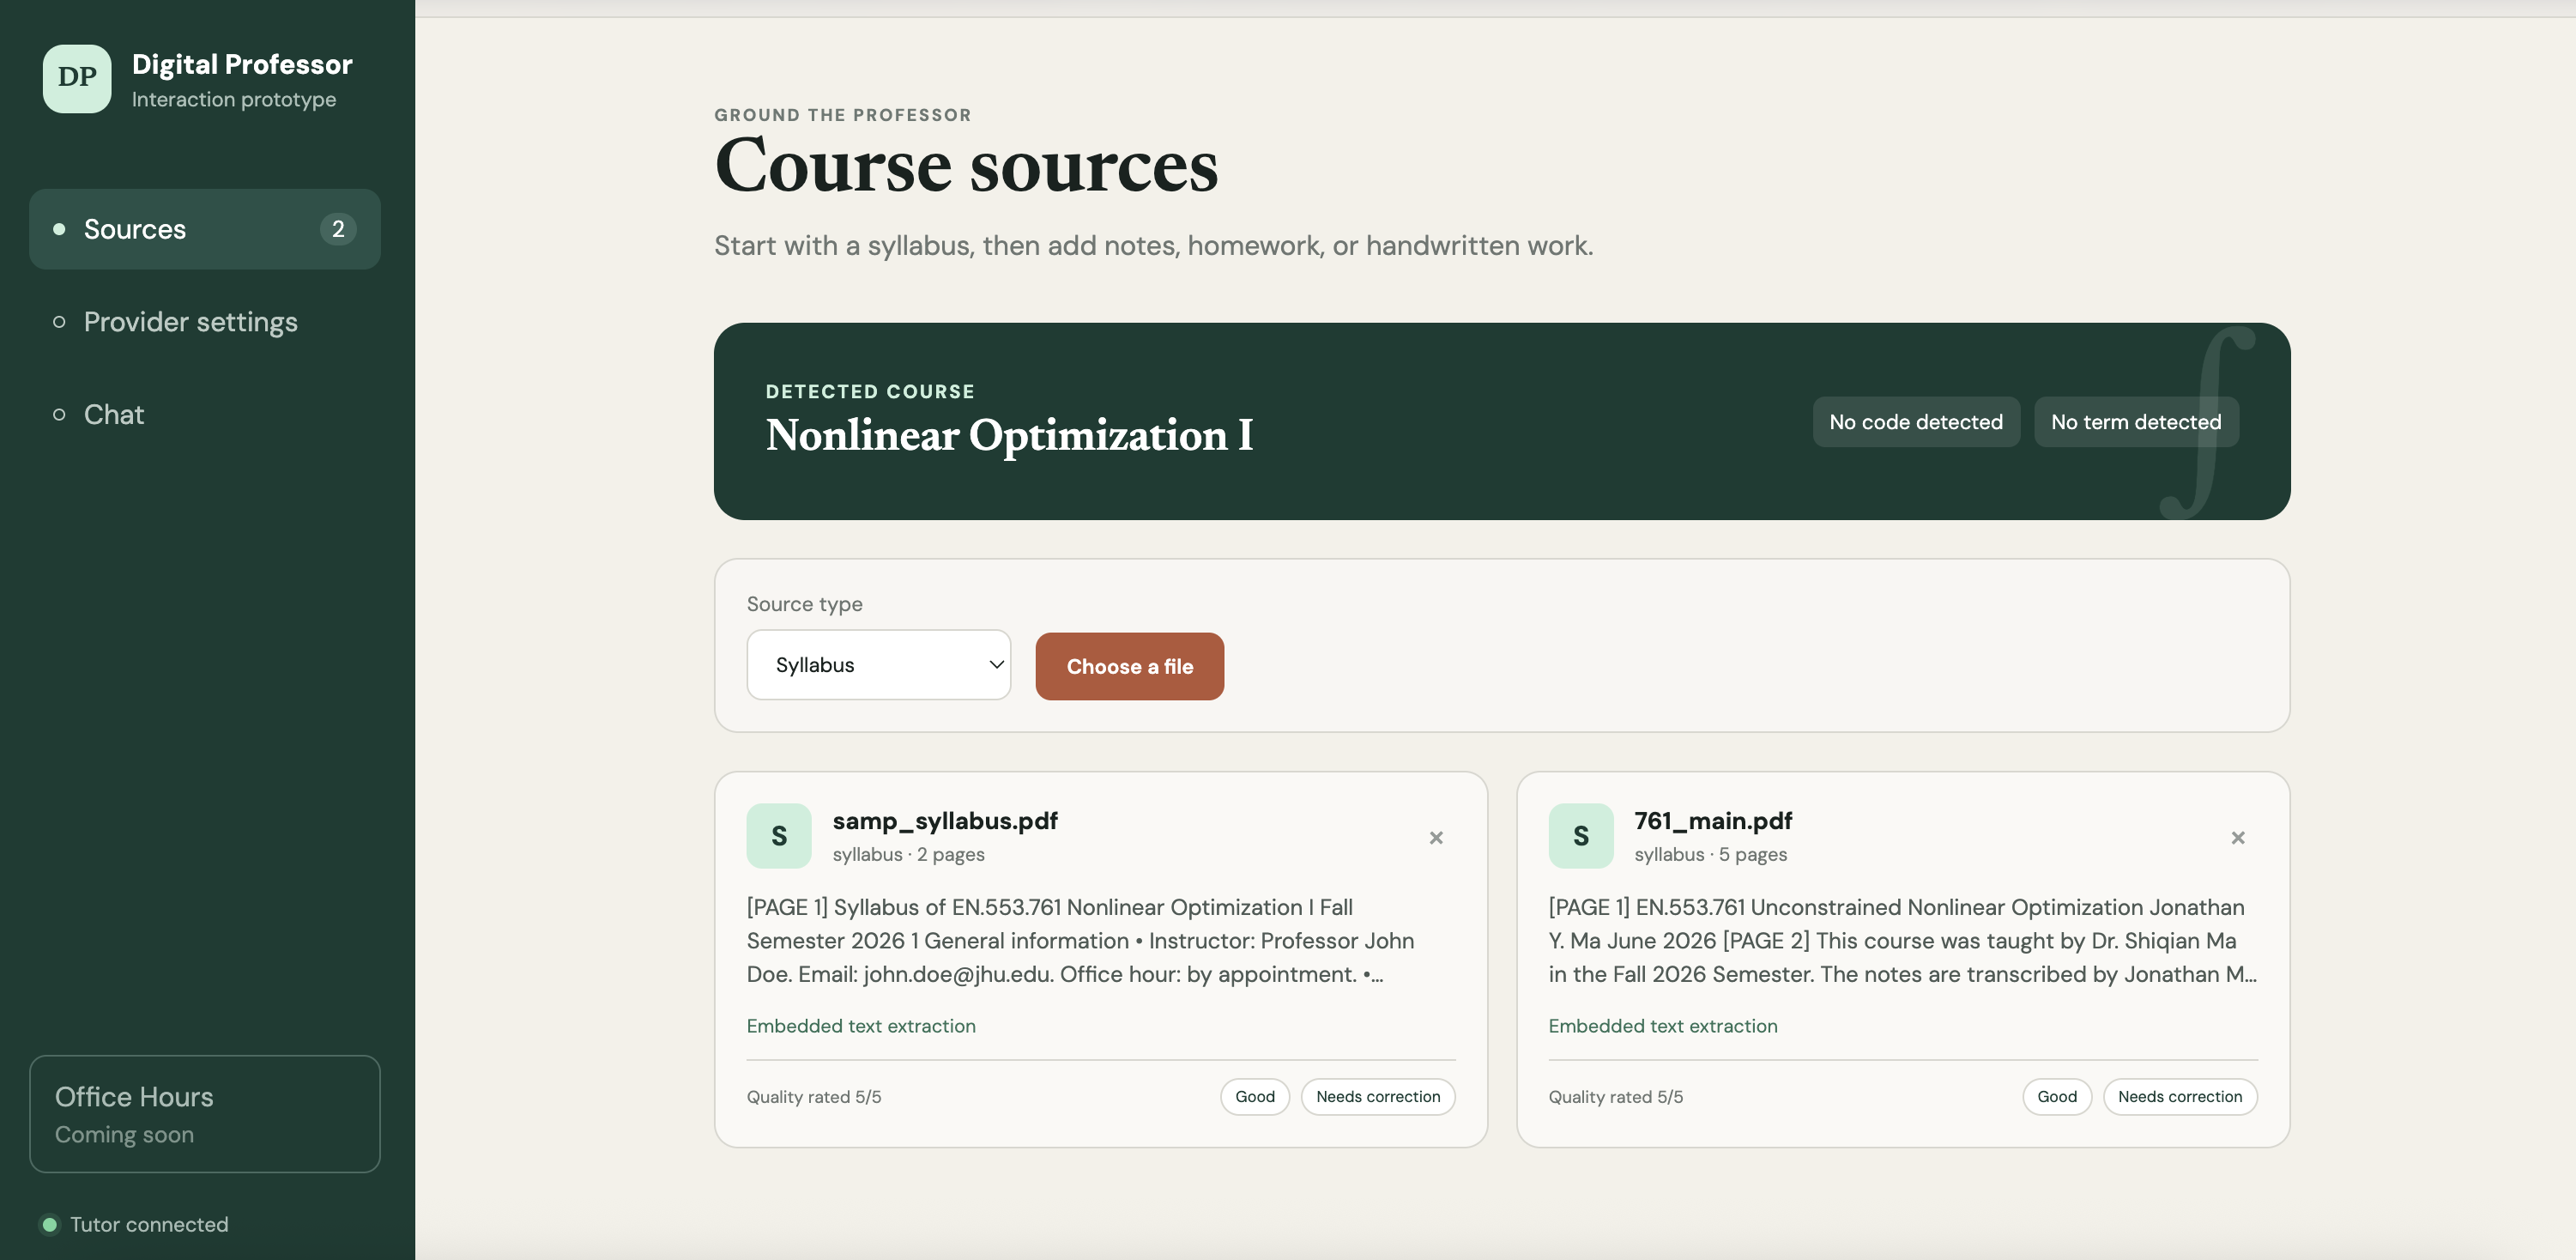
\includegraphics[width=\linewidth]{landing_and_upload.png}
    \column{0.29\textwidth}
      \footnotesize
      \textbf{Worked well}
      \begin{itemize}
        \item PDF upload was extracted in full
        \item Two PDFs were ingested and correctly classified as notes or syllabus
        \item Source method and quality controls are visible
      \end{itemize}
      \textbf{Did not work yet}
      \begin{itemize}
        \item Course code and term were not detected, sometimes Names cannot parse
        \item Internal page markers appear in the preview
        \item Metadata still needs an edit-and-confirm step
      \end{itemize}
  \end{columns}
\end{frame}

\begin{frame}{Demo evidence: configurable provider controls}
  \begin{columns}[T,onlytextwidth]
    \column{0.61\textwidth}
      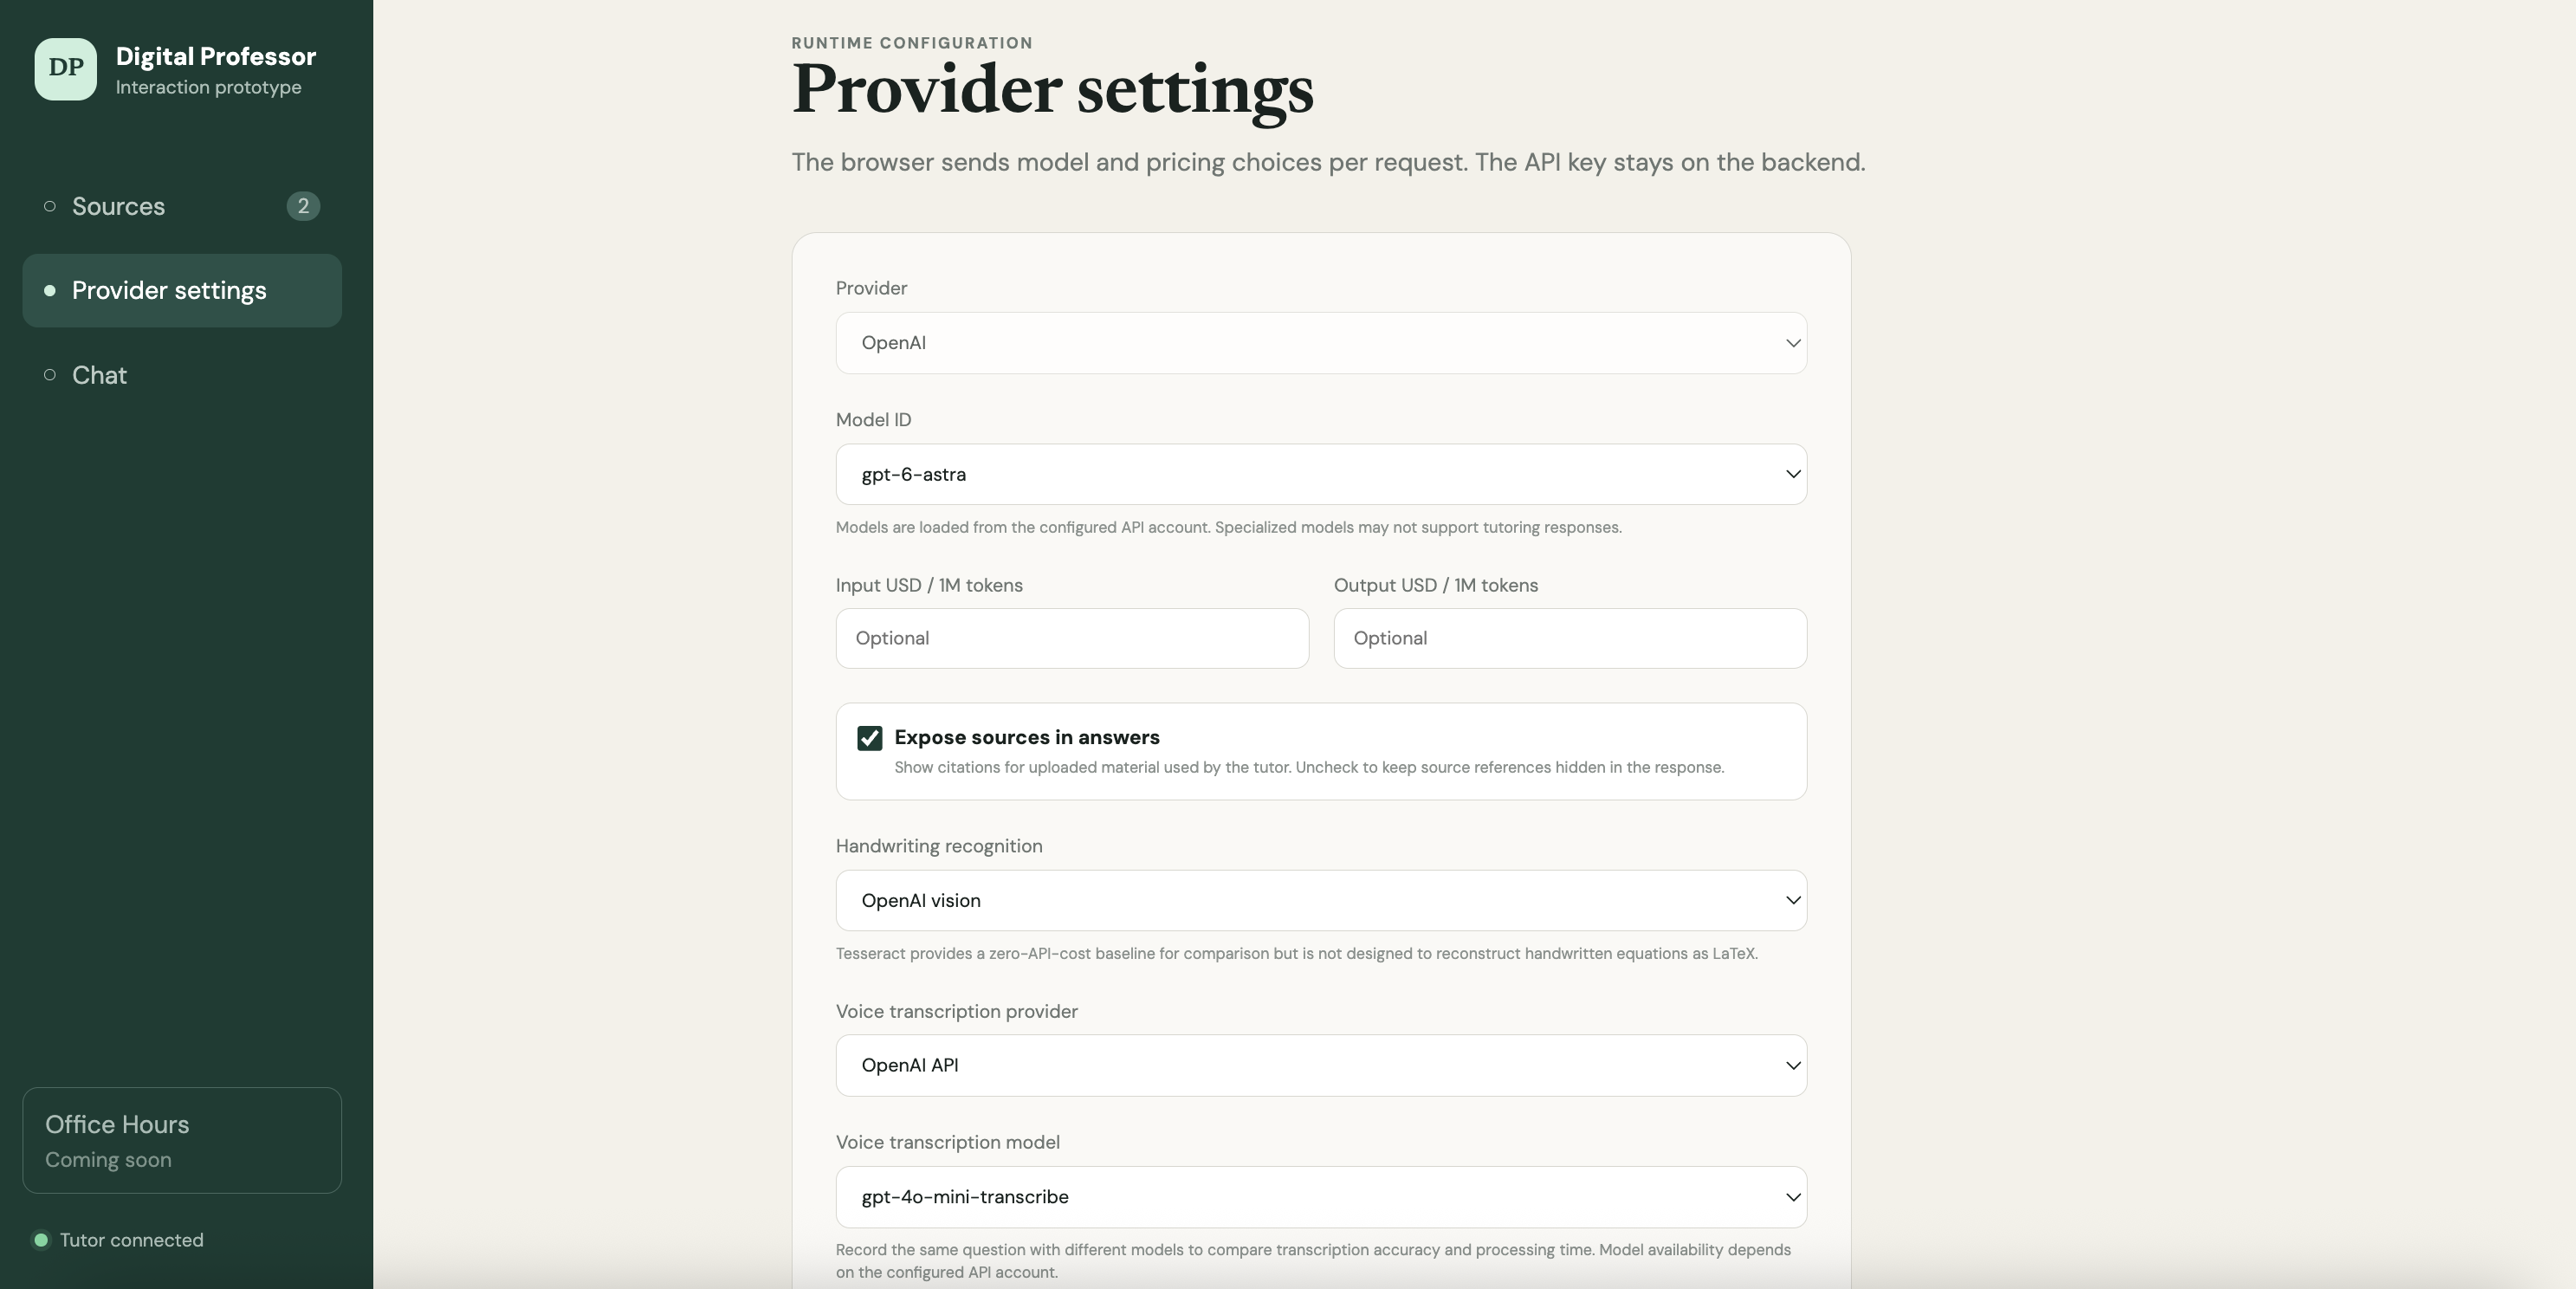
\includegraphics[width=\linewidth,height=2.75cm,keepaspectratio]{settings_1.png}\par
      \vspace{0.35em}
      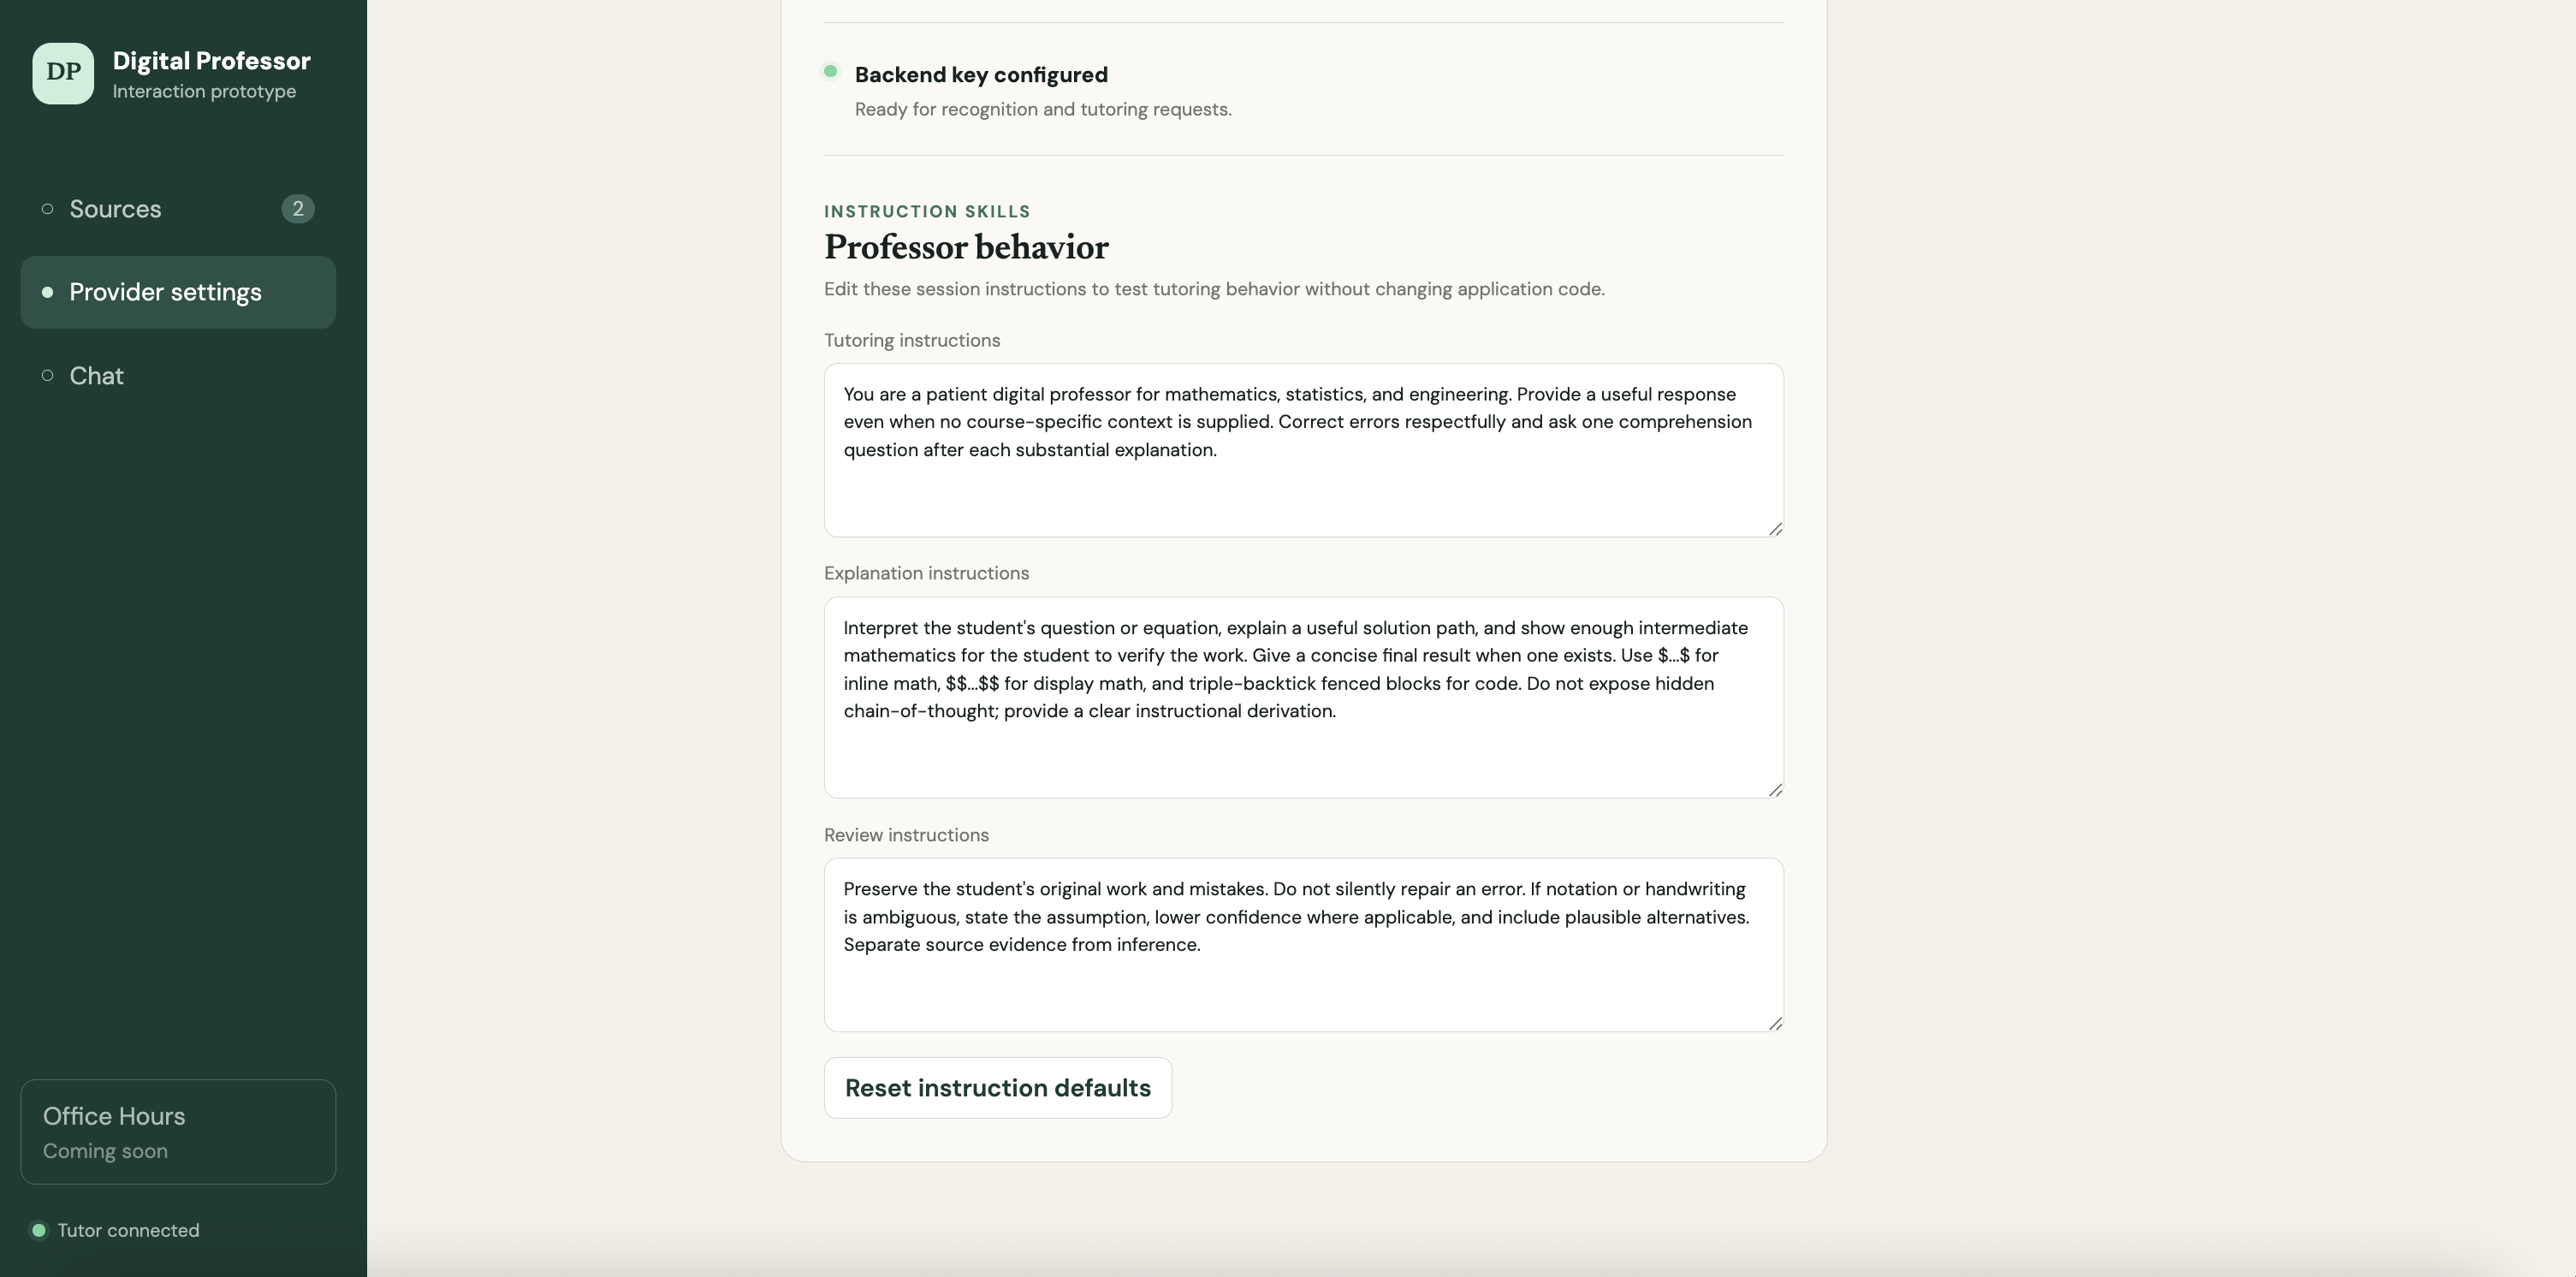
\includegraphics[width=\linewidth,height=2.75cm,keepaspectratio]{settings_2.png}
    \column{0.36\textwidth}
      \footnotesize
      \textbf{Worked well}
      \begin{itemize}
        \item Model, source exposure, handwriting, and voice controls are centralized
        \item API key status is visible without exposing the key
        \item Professor behavior is editable without code changes
      \end{itemize}
      \textbf{Still awkward}
      \begin{itemize}
        \item Settings require significant scrolling
        \item Token rates must be entered manually for cost estimates
        \item Some listed models may not support tutoring output
      \end{itemize}
  \end{columns}
\end{frame}

\begin{frame}{Student experience in the prototype}
  \centering
  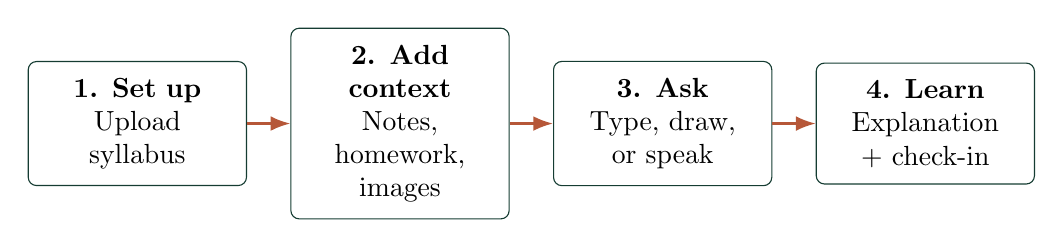
\begin{tikzpicture}[
    node distance=0.55cm,
    box/.style={draw=Forest, rounded corners=3pt, fill=white, minimum height=1.35cm,
      text width=2.35cm, align=center, inner sep=6pt},
    arrow/.style={-{Latex[length=2.5mm]}, thick, draw=Rust}
  ]
    \node[box] (setup) {\textbf{1. Set up}\\Upload syllabus};
    \node[box, right=of setup] (sources) {\textbf{2. Add context}\\Notes, homework, images};
    \node[box, right=of sources] (interact) {\textbf{3. Ask}\\Type, draw, or speak};
    \node[box, right=of interact] (response) {\textbf{4. Learn}\\Explanation + check-in};
    \draw[arrow] (setup) -- (sources);
    \draw[arrow] (sources) -- (interact);
    \draw[arrow] (interact) -- (response);
  \end{tikzpicture}
  \vspace{1em}
  \begin{itemize}
    \item The syllabus supplies a proposed course name, code, and term.
    \item Uploaded material becomes context for later chat requests.
    \item Transcriptions and recognized handwriting remain visible for review.
    \item The tutor explains its assumptions and asks whether the student follows.
  \end{itemize}
\end{frame}

\begin{frame}{Prototype architecture}
  \begin{columns}[T,onlytextwidth]
    \column{0.58\textwidth}
      \centering
      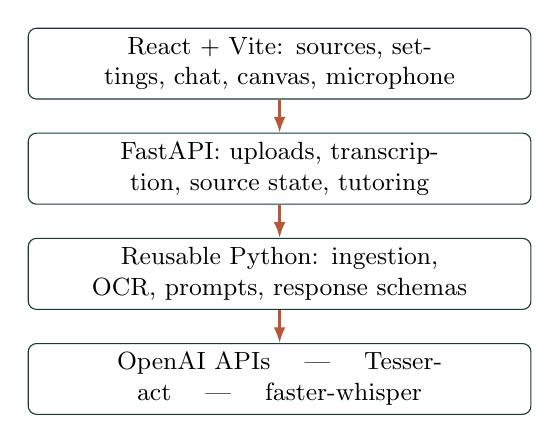
\begin{tikzpicture}[
        node distance=0.42cm,
        layer/.style={draw=Forest, rounded corners=3pt, fill=white, text width=6.15cm,
          minimum height=0.85cm, align=center, font=\small},
        arrow/.style={-{Latex[length=2mm]}, thick, draw=Rust}
      ]
        \node[layer] (ui) {React + Vite: sources, settings, chat, canvas, microphone};
        \node[layer, below=of ui] (api) {FastAPI: uploads, transcription, source state, tutoring};
        \node[layer, below=of api] (services) {Reusable Python: ingestion, OCR, prompts, response schemas};
        \node[layer, below=of services] (providers) {OpenAI APIs \quad | \quad Tesseract \quad | \quad faster-whisper};
        \draw[arrow] (ui) -- (api);
        \draw[arrow] (api) -- (services);
        \draw[arrow] (services) -- (providers);
      \end{tikzpicture}
    \column{0.39\textwidth}
      \begin{itemize}
        \item Browser-based and currently run on localhost
        \item API key stays on the backend
        \item Research code is isolated under \texttt{research/}\allowbreak\texttt{interaction-methods}
        \item Tutoring, explanation, and review instructions live in a configurable skills file
        \item In-memory state keeps iteration simple
      \end{itemize}
  \end{columns}
\end{frame}

\begin{frame}{Demo evidence: tutoring chat}
  \begin{columns}[T,onlytextwidth]
    \column{0.495\textwidth}
      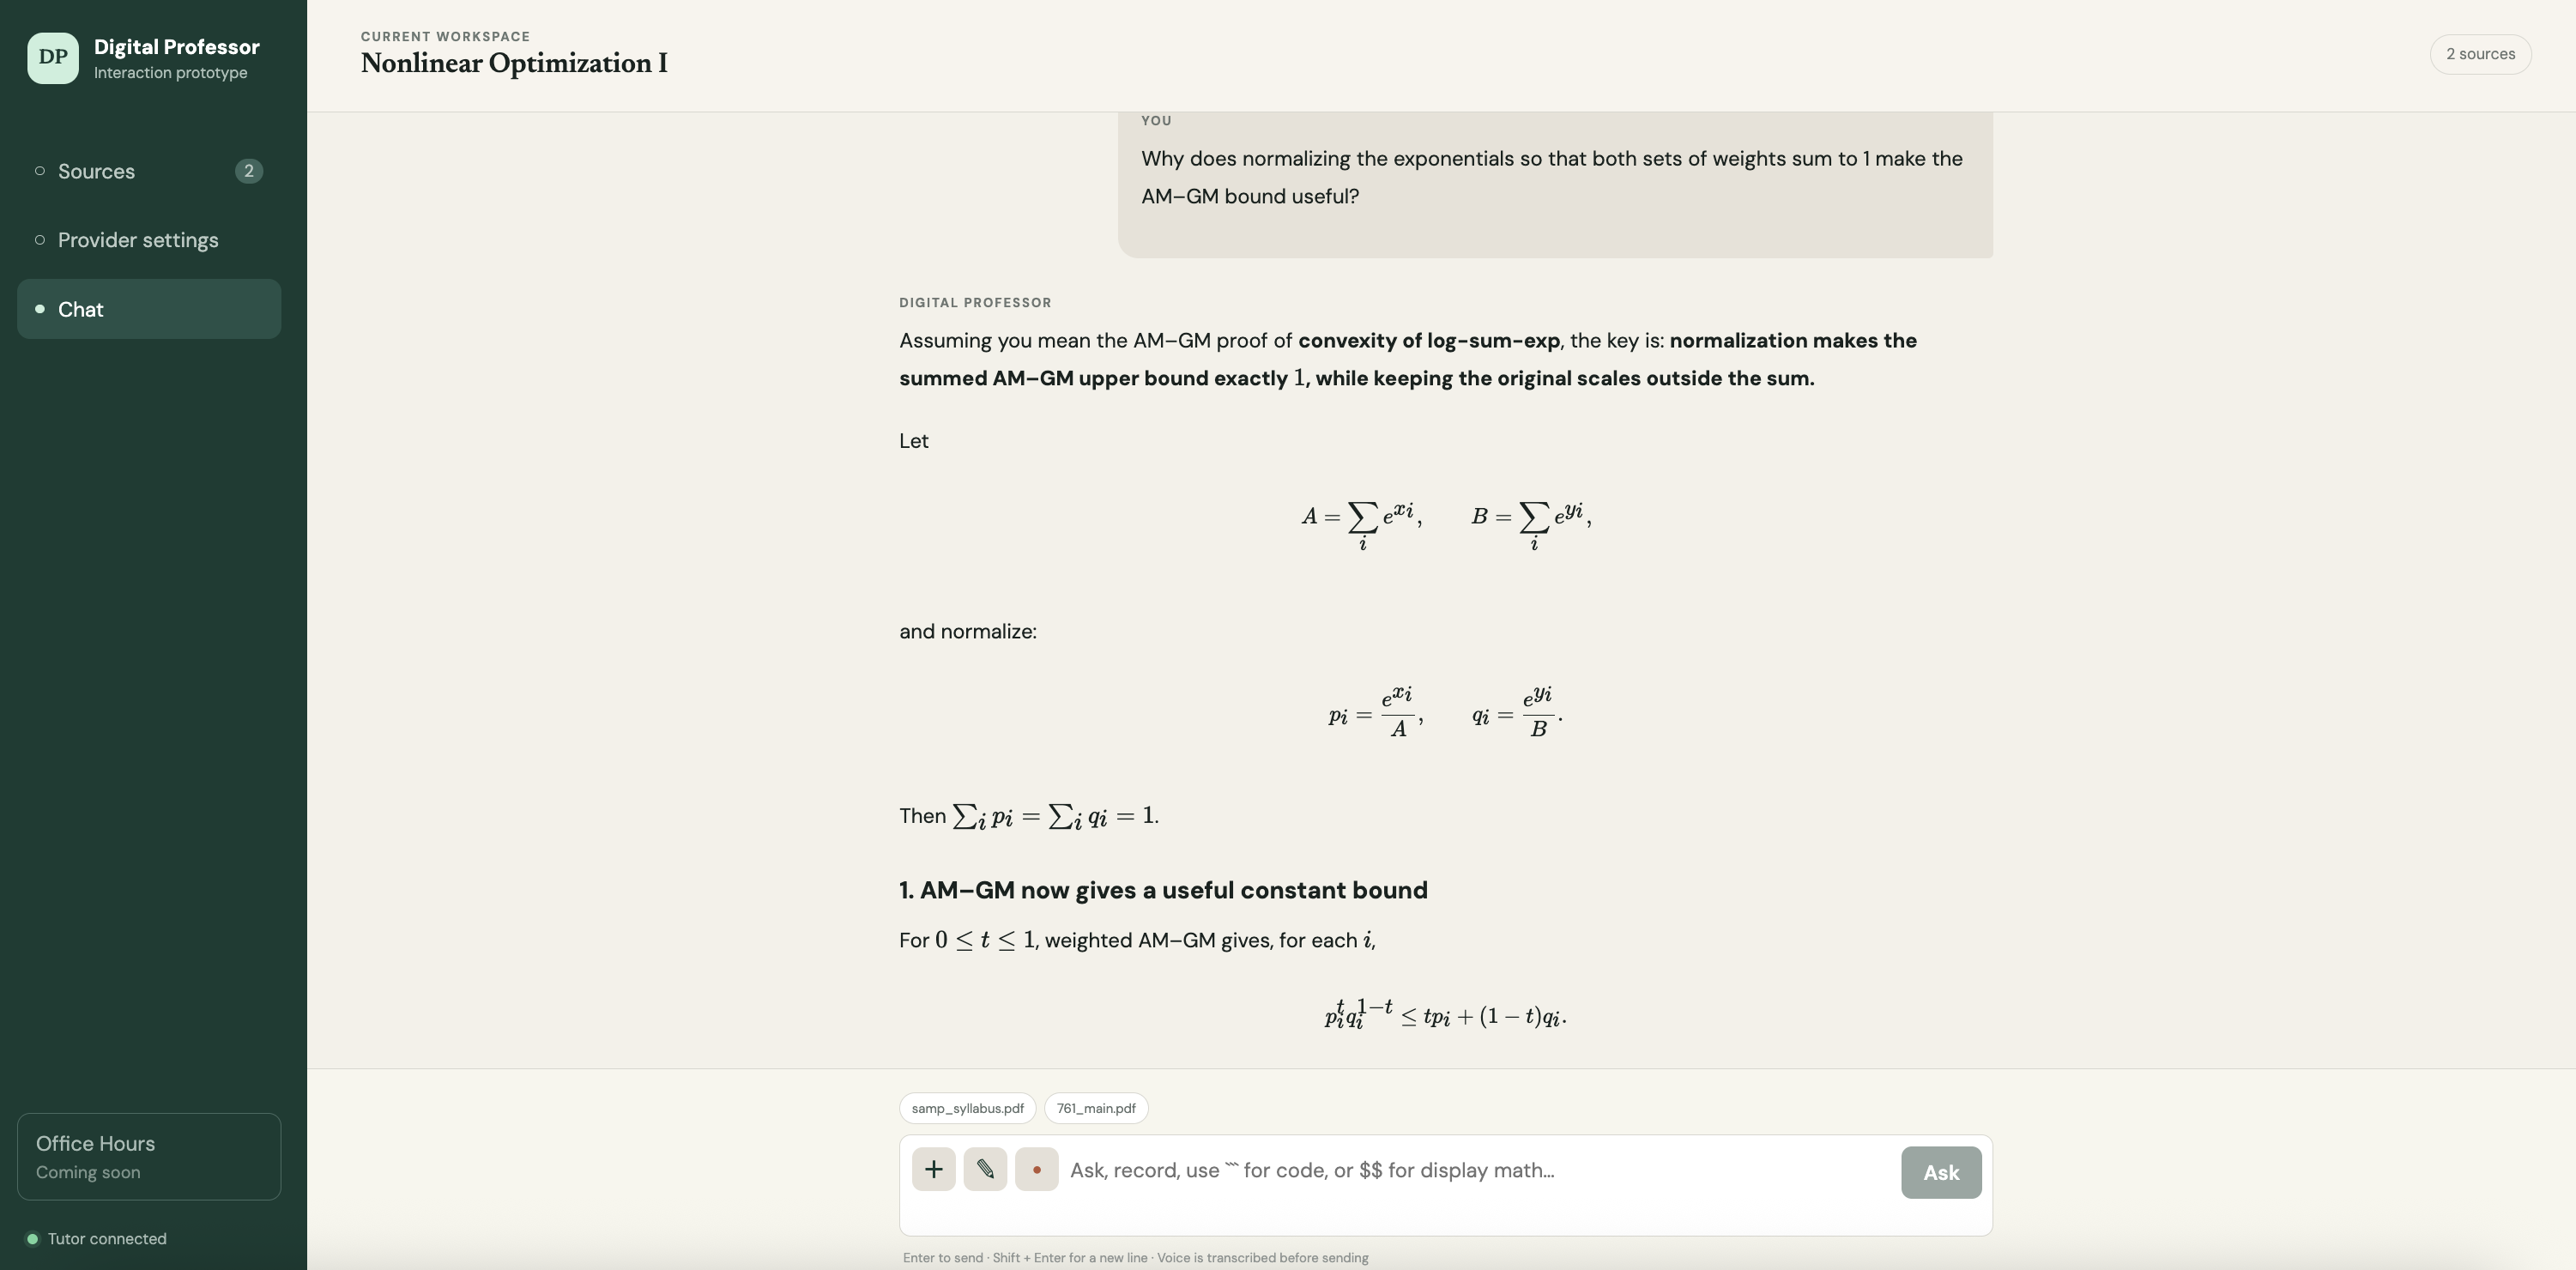
\includegraphics[width=\linewidth]{chat_1.png}
    \column{0.495\textwidth}
      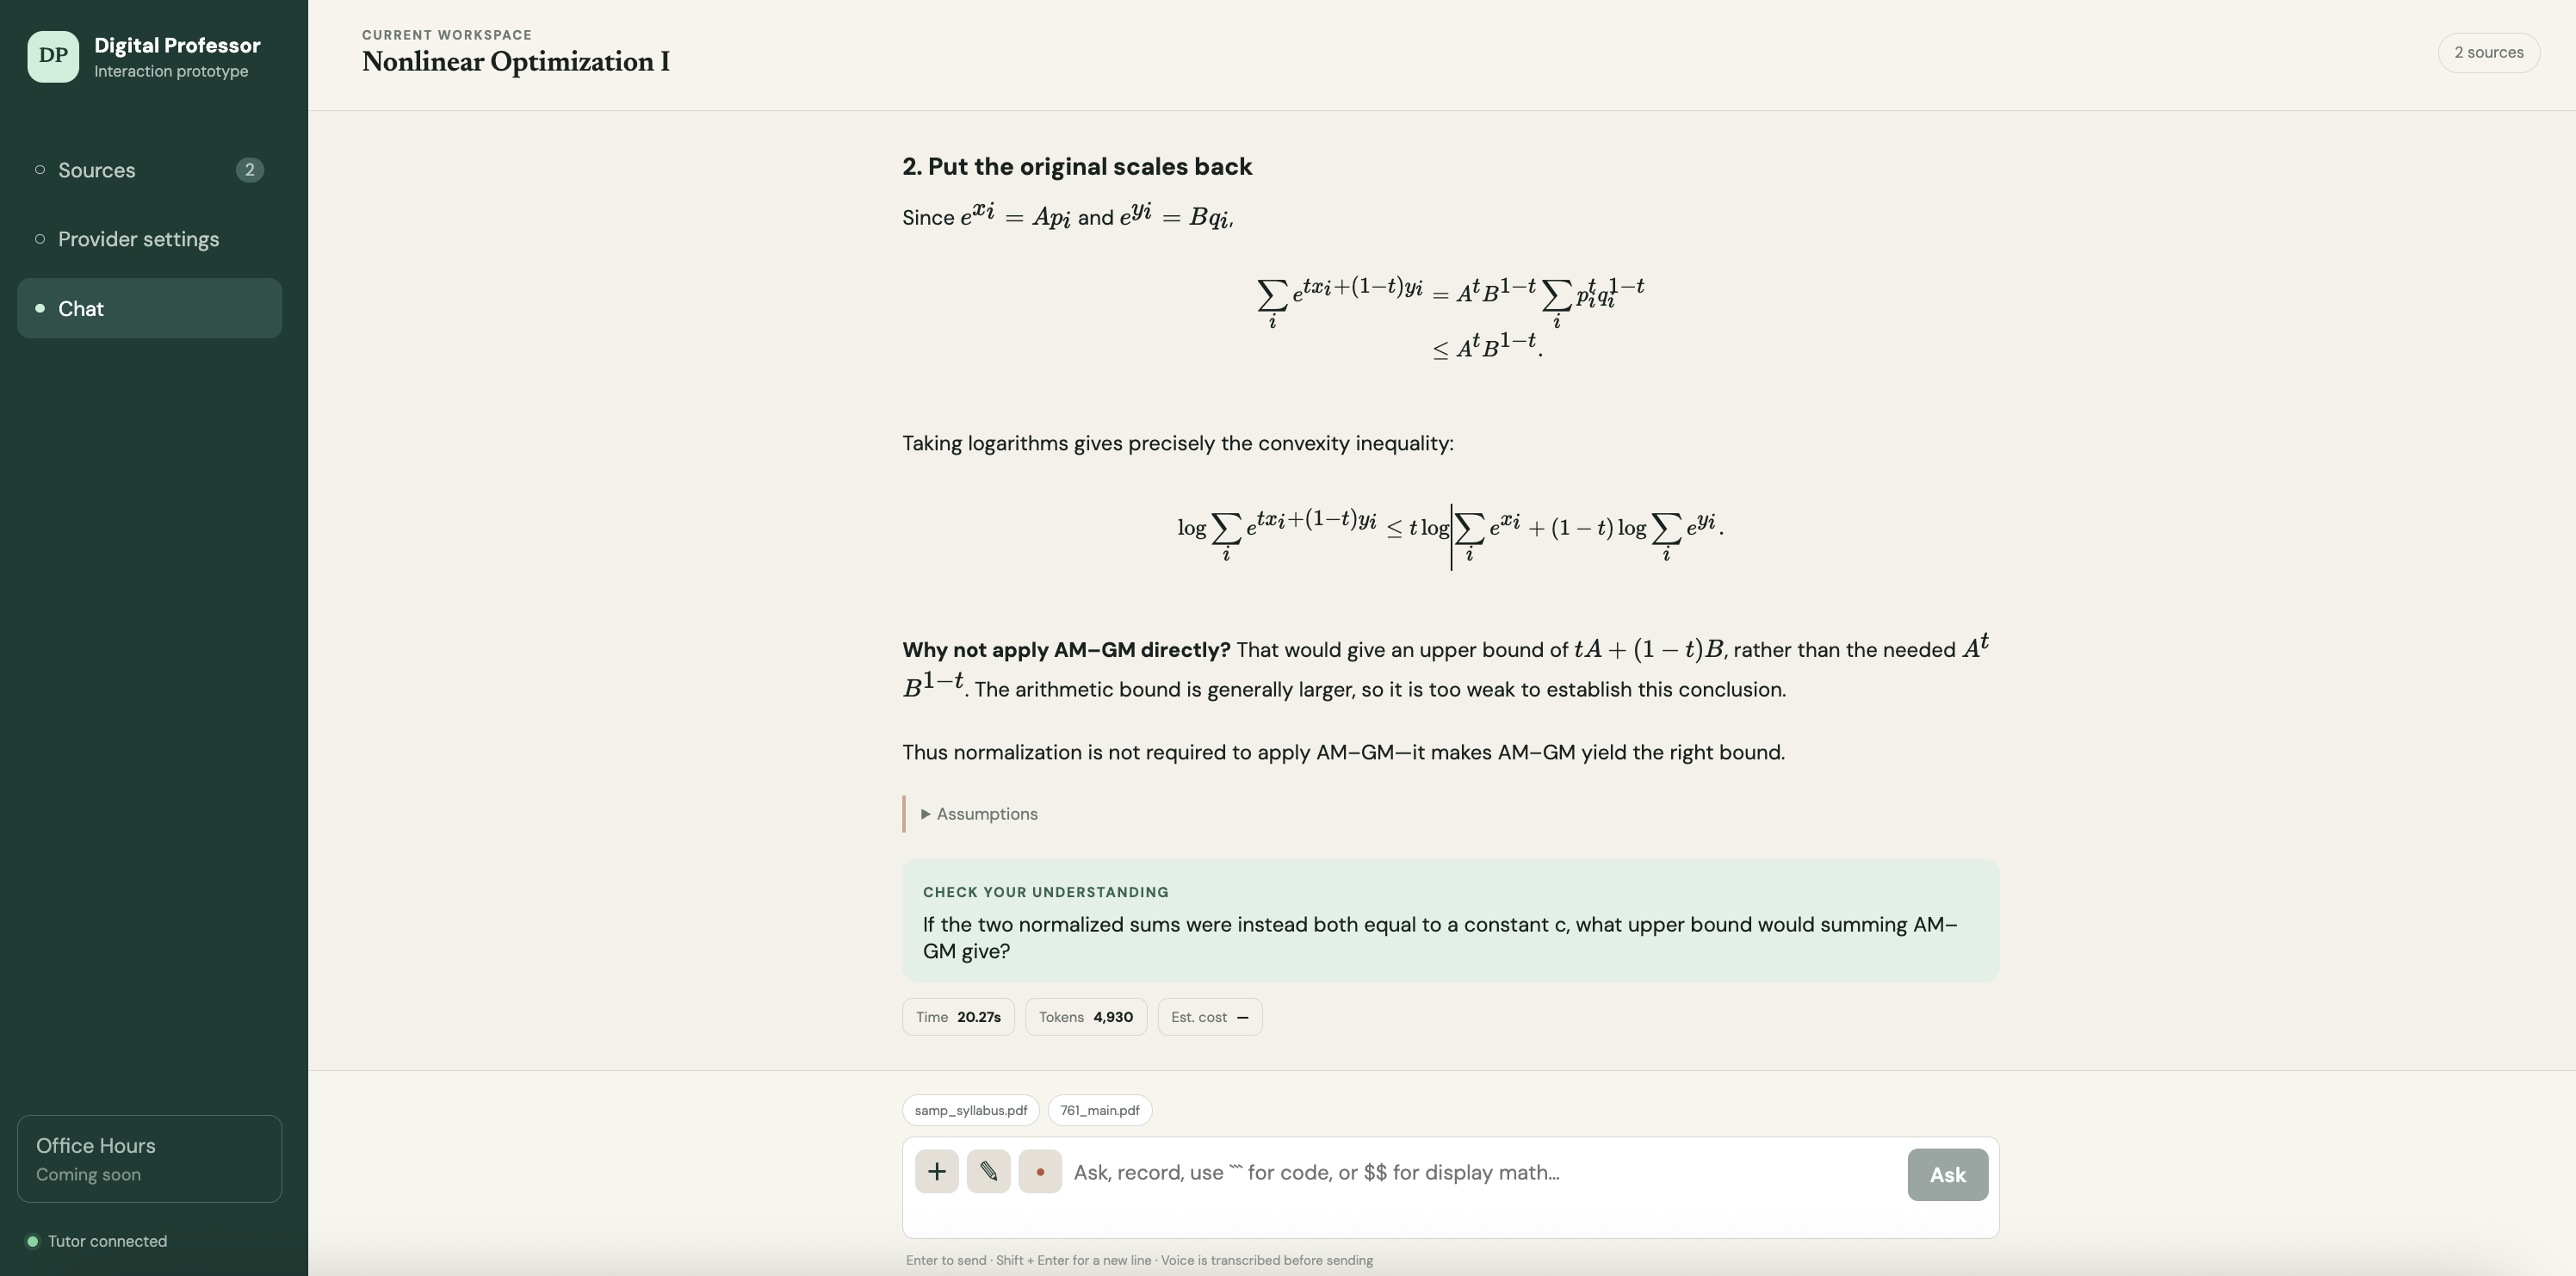
\includegraphics[width=\linewidth]{chat_2.png}
  \end{columns}
  \vspace{0.45em}
  \begin{columns}[T,onlytextwidth]
    \column{0.49\textwidth}
      \textbf{Worked well}
      \begin{itemize}
        \item Course-specific question produced a worked response
        \item Display equations rendered cleanly
        \item Assumptions, comprehension check, source chips, and metrics are present
      \end{itemize}
    \column{0.47\textwidth}
      \textbf{Needs improvement}
      \begin{itemize}
        \item Answer is long and requires substantial scrolling
        \item Example latency is about 20 seconds
        \item Estimated cost is blank until token rates are configured
        \item Citation visibility and correctness need live-demo validation
      \end{itemize}
  \end{columns}
\end{frame}

\begin{frame}{Document ingestion}
  \begin{columns}[T,onlytextwidth]
    \column{0.53\textwidth}
      \textbf{Implemented pipeline}
      \begin{enumerate}
        \item Accept PDF, text, Markdown, \TeX{}, PNG, JPEG, and WebP
        \item Extract embedded PDF text locally with PyMuPDF
        \item Detect image-only or low-text PDFs
        \item Render pages and route them to visual recognition
        \item Store normalized text as chat context
      \end{enumerate}
    \column{0.43\textwidth}
      \begin{block}{Recognition comparison}
        \begin{itemize}
          \item OpenAI vision for handwriting and mathematical notation
          \item Tesseract as a zero-API-cost OCR baseline
          \item Per-request method and elapsed time recorded
        \end{itemize}
      \end{block}
      \risk{Current gap:} citations preserve available page markers, but citation correctness and retrieval quality are not yet formally evaluated.
  \end{columns}
\end{frame}

\begin{frame}{Live writing and handwriting recognition}
  \begin{columns}[T,onlytextwidth]
    \column{0.50\textwidth}
      \textbf{What works}
      \begin{itemize}
        \item Sketchpad opens directly from the chat composer
        \item Mouse, touch, Apple Pencil, and compatible stylus input
        \item Adjustable pen width, clear, cancel, and upload controls
        \item Canvas exports a PNG into the existing ingestion pipeline
        \item Works across desktop and local-network mobile testing
      \end{itemize}
    \column{0.46\textwidth}
      \textbf{What this lets us test}
      \begin{itemize}
        \item Natural handwritten questions
        \item Ambiguous symbols and notation
        \item Equations that are difficult to type
        \item OpenAI vision versus Tesseract output
      \end{itemize}
      \vspace{0.4em}
      \risk{Known limitation:} Tesseract is designed mainly for printed text and does not reliably reconstruct 2-D math as \TeX{}.
  \end{columns}
\end{frame}

\begin{frame}{Simple voice recording and transcription}
  \begin{columns}[T,onlytextwidth]
    \column{0.49\textwidth}
      \textbf{Interaction}
      \begin{itemize}
        \item Start and stop recording from the chat composer
        \item Convert speech to editable text before submission
        \item Use a file/capture fallback when mobile browsers block recording
        \item Accept common audio formats up to the demo upload limit
      \end{itemize}
    \column{0.47\textwidth}
      \textbf{Testable providers}
      \begin{itemize}
        \item OpenAI: GPT Transcribe, GPT-4o Transcribe, mini, and Whisper-1
        \item Local faster-whisper: tiny, base, and small
        \item Report provider, model, and transcription time
      \end{itemize}
      \vspace{0.4em}
      \risk{Known limitation:} microphone capture on a phone generally requires HTTPS; plain LAN HTTP uses the recording/file fallback.
  \end{columns}
\end{frame}

\begin{frame}{Source exposure and evaluation telemetry}
  \begin{columns}[T,onlytextwidth]
    \column{0.49\textwidth}
      \textbf{Source exposure}
      \begin{itemize}
        \item Provider setting shows or hides citations in answers
        \item Structured citation: validated source ID, filename, optional page, and supporting basis
        \item Unknown or fabricated source IDs are removed by the backend
        \item Page markers are preserved during ingestion when available
      \end{itemize}
    \column{0.47\textwidth}
      \textbf{Research telemetry}
      \begin{itemize}
        \item JSONL log plus a read-only session metrics endpoint
        \item Latency, tokens, configured cost, provider, and model
        \item Equation-confidence proxy and student quality rating
        \item Edit distance and correction rate for voice drafts
        \item Citation count and source-exposure state
      \end{itemize}
  \end{columns}
  \vspace{0.35em}
  \good{Privacy boundary:} logs contain metrics and identifiers; they exclude source contents, transcripts, questions, and answers.
\end{frame}

\begin{frame}{What still needs to get done}
  \small
  \begin{tabular}{p{0.25\textwidth}p{0.42\textwidth}p{0.24\textwidth}}
    \toprule
    \textbf{Area} & \textbf{Next deliverable} & \textbf{Why it matters} \\
    \midrule
    Evaluation & Fixed test set, ground truth, accuracy, latency, and cost comparison & Select providers with evidence \\
    Grounding & Chunking, retrieval, citation evaluation, and source previews & Make answers auditable \\
    Course setup & AI-assisted syllabus extraction with editable metadata & Reduce setup friction \\
    Persistence & Database, course workspaces, chat history, and file storage & Support repeat use \\
    Product safety & Authentication, privacy controls, retention rules, moderation & Prepare for real students \\
    Accessibility & Keyboard paths, captions, screen-reader checks, contrast testing & Support diverse learners \\
    \bottomrule
  \end{tabular}
\end{frame}

\begin{frame}{Blockers and risks}
  \begin{columns}[T,onlytextwidth]
    \column{0.49\textwidth}
      \begin{block}{Technical blockers}
        \begin{itemize}
          \item Local OCR/transcription tools require optional native packages and model downloads
          \item Mobile microphone access needs trusted HTTPS
          \item Provider model access and behavior vary by API account
          \item Current state disappears when the backend restarts
        \end{itemize}
      \end{block}
    \column{0.49\textwidth}
      \begin{block}{Research risks}
        \begin{itemize}
          \item Handwriting and spoken math remain highly ambiguous
          \item A fluent answer may still be mathematically wrong
          \item More agents add cost and failure points without proven need
          \item Student data introduces privacy and consent requirements
        \end{itemize}
      \end{block}
  \end{columns}
  \vspace{0.3em}
  \good{Mitigation direction:} retain editable intermediate outputs, expose assumptions, cite sources, and evaluate every modality on the same tasks.
\end{frame}

\begin{frame}{Roadmap}
  \begin{enumerate}
    \item[\textbf{1}] \textbf{Measure the current prototype} \hfill \textcolor{Muted}{Next}
      \begin{itemize}
        \item Run identical document, handwriting, equation, and audio samples across providers
        \item Add ground truth and scoring to the metrics already captured
      \end{itemize}
    \item[\textbf{2}] \textbf{Make course grounding dependable}
      \begin{itemize}
        \item Add retrieval, validate page citations, editable course metadata, persistence, and tests
      \end{itemize}
    \item[\textbf{3}] \textbf{Pilot a secure public web application}
      \begin{itemize}
        \item Add HTTPS, authentication, storage, privacy controls, and observability
      \end{itemize}
    \item[\textbf{4}] \textbf{Prototype Office Hours after chat evaluation}
      \begin{itemize}
        \item Real-time voice, optional video/avatar, interruption handling, transcript, and shared canvas
      \end{itemize}
    \item[\textbf{5}] \textbf{Add manager--worker agents only where evaluation shows value}
      \begin{itemize}
        \item Candidate workers: document ingestion, math handling, tablet input, and transcription
      \end{itemize}
  \end{enumerate}
\end{frame}

\begin{frame}{Recommended next milestone}
  \begin{block}{Deliver a measured interaction demo}
    One student task should move through typed input, a source document, handwriting, and voice while the prototype records recognition quality, correction effort, response quality, latency, and cost.
  \end{block}
  \vspace{0.8em}
  \begin{itemize}
    \item Demonstrates the complete value proposition without committing to Office Hours architecture
    \item Produces evidence for provider and model selection
    \item Reveals whether specialized agents are needed
    \item Creates a clear acceptance gate for deployment work
  \end{itemize}
  \vfill
  \centering\Large\color{Forest}\textbf{Questions and prototype walkthrough}
\end{frame}

\end{document}
